% Created 2021-10-28 Thu 00:58
% Intended LaTeX compiler: pdflatex
\documentclass[11pt]{article}
\usepackage[utf8]{inputenc}
\usepackage[T1]{fontenc}
\usepackage{graphicx}
\usepackage{grffile}
\usepackage{longtable}
\usepackage{wrapfig}
\usepackage{rotating}
\usepackage[normalem]{ulem}
\usepackage{amsmath}
\usepackage{textcomp}
\usepackage{amssymb}
\usepackage{capt-of}
\usepackage{hyperref}
\usepackage{minted}
\usepackage{amsfonts}
\usepackage{physics}
\author{Justice Sefas}
\date{\today}
\title{HW3}
\hypersetup{
 pdfauthor={Justice Sefas},
 pdftitle={HW3},
 pdfkeywords={},
 pdfsubject={},
 pdfcreator={Emacs 27.2 (Org mode 9.5)}, 
 pdflang={English}}
\begin{document}

\maketitle


\section*{Program 1}
\label{sec:org4245d85}
\subsection*{HMC}
\label{sec:org2638ba9}
\subsubsection*{Plots}
\label{sec:org2dff762}
\begin{center}
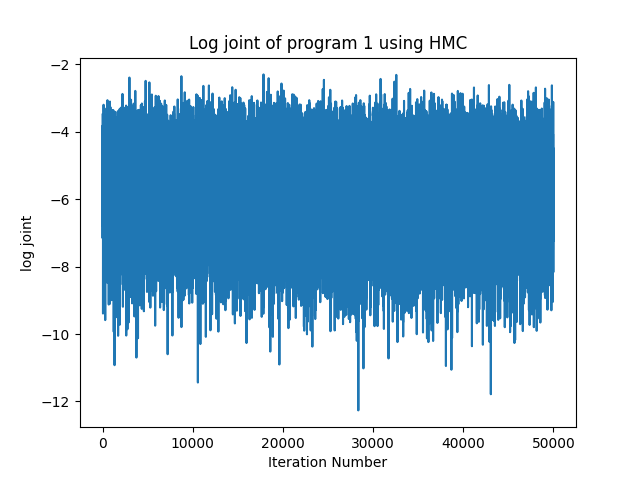
\includegraphics[width=.9\linewidth]{/home/jsefas/probprog/cpsc532w-hw2/joint-density-1-HMC.png}
\end{center}
\begin{center}
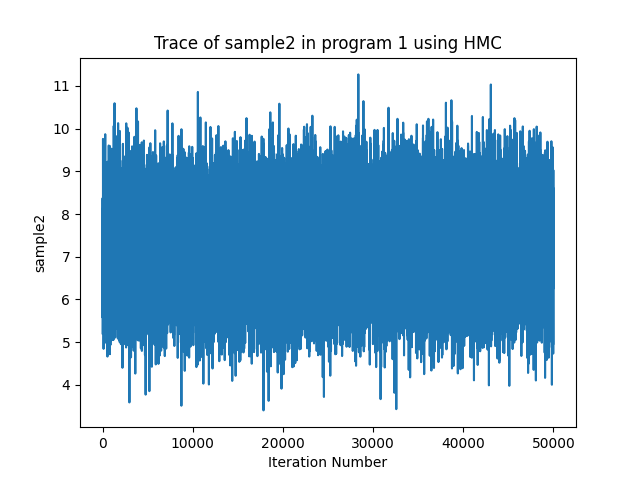
\includegraphics[width=.9\linewidth]{/home/jsefas/probprog/cpsc532w-hw2/trace-sample2-1-HMC.png}
\end{center}
\subsubsection*{Run time (s)}
\label{sec:org8a77829}
350.9575340747833
\subsubsection*{Mean}
\label{sec:org84d55d2}
7.23814616
\subsubsection*{Variance}
\label{sec:org6a574b3}
0.82865091

\subsection*{Gibbs}
\label{sec:org2375f22}
\subsubsection*{Plots}
\label{sec:org32cc8c8}
\begin{center}
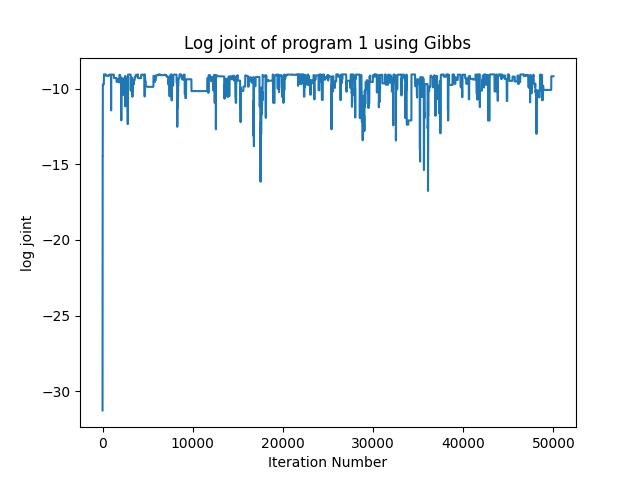
\includegraphics[width=.9\linewidth]{/home/jsefas/probprog/cpsc532w-hw2/joint-density-1-Gibbs.png}
\end{center}
\begin{center}
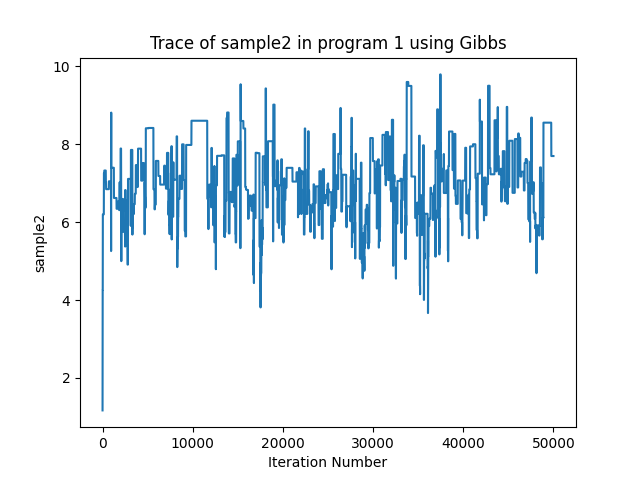
\includegraphics[width=.9\linewidth]{/home/jsefas/probprog/cpsc532w-hw2/trace-sample2-1-Gibbs.png}
\end{center}

\subsubsection*{Run time (s)}
\label{sec:orgd453c7b}
45.406129598617554
\subsubsection*{Mean}
\label{sec:org03c64a4}
7.17261325
\subsubsection*{Variance}
\label{sec:org17f03c7}
8.32507872e-01

\subsection*{Importance Sampling}
\label{sec:orgd29a7f3}

\section*{Program 2}
\label{sec:orgff6443d}
\subsection*{HMC}
\label{sec:org0fa3f50}
\begin{center}
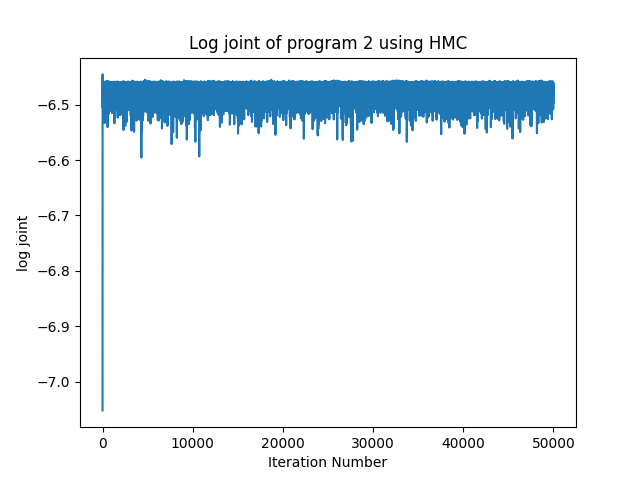
\includegraphics[width=.9\linewidth]{/home/jsefas/probprog/cpsc532w-hw2/joint-density-2-HMC.png}
\end{center}
\begin{center}
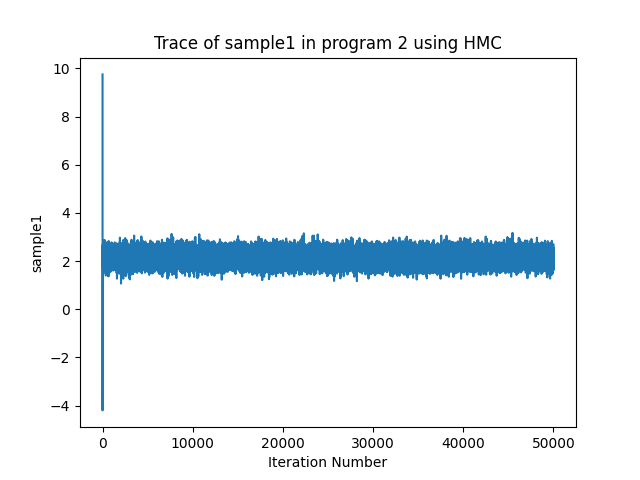
\includegraphics[width=.9\linewidth]{/home/jsefas/probprog/cpsc532w-hw2/trace-sample1-2-HMC.png}
\end{center}
\begin{center}
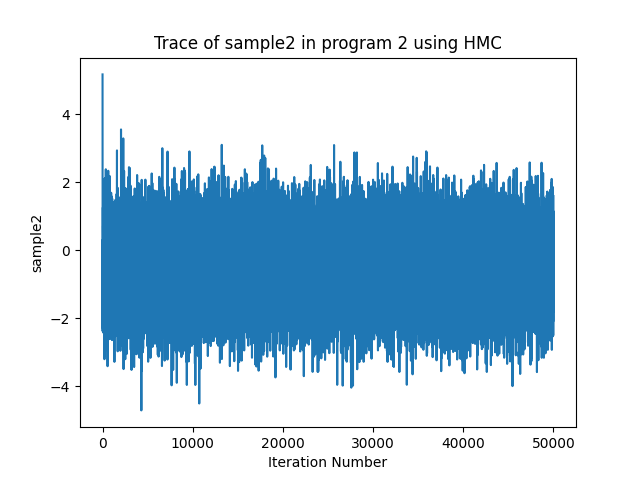
\includegraphics[width=.9\linewidth]{/home/jsefas/probprog/cpsc532w-hw2/trace-sample2-2-HMC.png}
\end{center}

\subsection*{Gibbs}
\label{sec:org13edd46}
\begin{center}
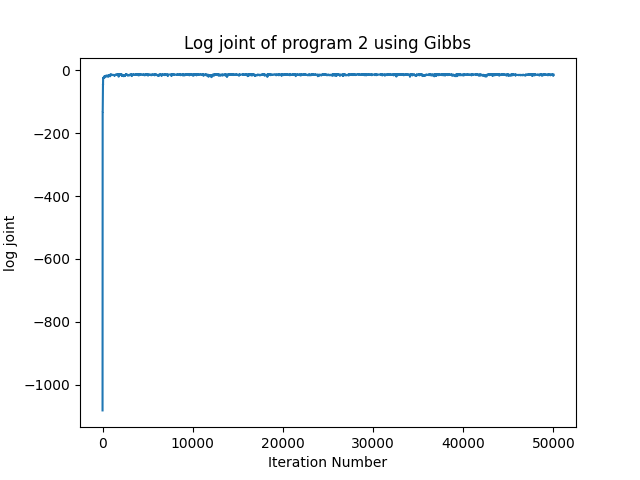
\includegraphics[width=.9\linewidth]{/home/jsefas/probprog/cpsc532w-hw2/joint-density-2-Gibbs.png}
\end{center}
\begin{center}
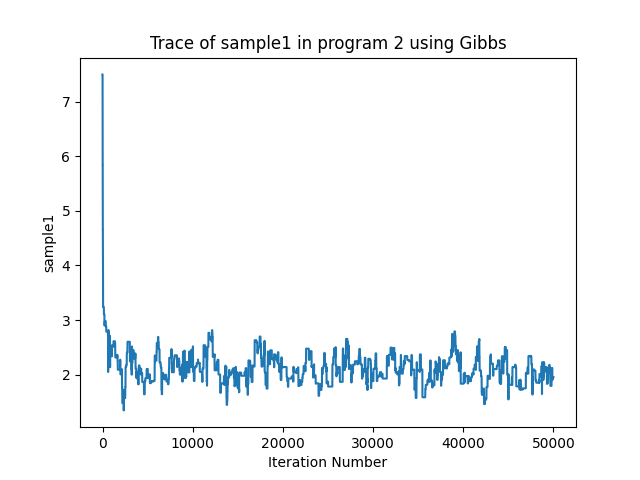
\includegraphics[width=.9\linewidth]{/home/jsefas/probprog/cpsc532w-hw2/trace-sample1-2-Gibbs.png}
\end{center}
\begin{center}
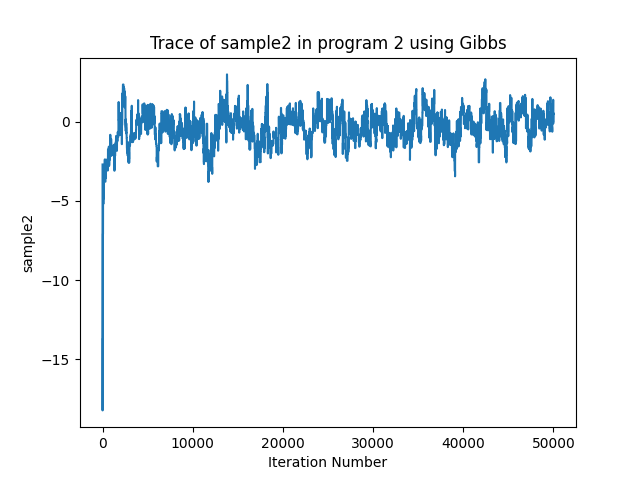
\includegraphics[width=.9\linewidth]{/home/jsefas/probprog/cpsc532w-hw2/trace-sample2-2-Gibbs.png}
\end{center}
\subsubsection*{Run time (s)}
\label{sec:org916bd72}
186.18388175964355
\subsubsection*{Mean}
\label{sec:org38480a2}
\begin{bmatrix}
2.11975777 & -0.41269691
\end{bmatrix}

\subsection*{Importance Sampling}
\label{sec:org00bd19d}
\subsubsection*{Run time (s)}
\label{sec:orgda9f76f}
55.23421025276184
\subsubsection*{Mean}
\label{sec:org020831d}
\begin{bmatrix}
2.1270 & -0.4365
\end{bmatrix}
\subsubsection*{Covariance}
\label{sec:orgbb93b32}
\begin{bmatrix}
0.05088208 & -0.18123494 \\
-0.18123494 & 0.82379968
\end{bmatrix}

\section*{Program 3}
\label{sec:org20cb6ae}
\subsection*{Gibbs}
\label{sec:org3dbbff8}
\subsection*{Importance}
\label{sec:orgf87571e}
\subsubsection*{Run time (s)}
\label{sec:orge0d774e}
73.02027440071106
\subsubsection*{Probability}
\label{sec:org2196cc9}
0.8041344881057739
\subsubsection*{Variance}
\label{sec:org2c9ffc0}
0.15750189558993366


\section*{Program 4}
\label{sec:org7e79bed}
\subsection*{Gibbs}
\label{sec:org7050a10}

\section*{Program 5}
\label{sec:orgb4dc8cb}
\subsection*{HMC}
\label{sec:org172406f}
\begin{center}
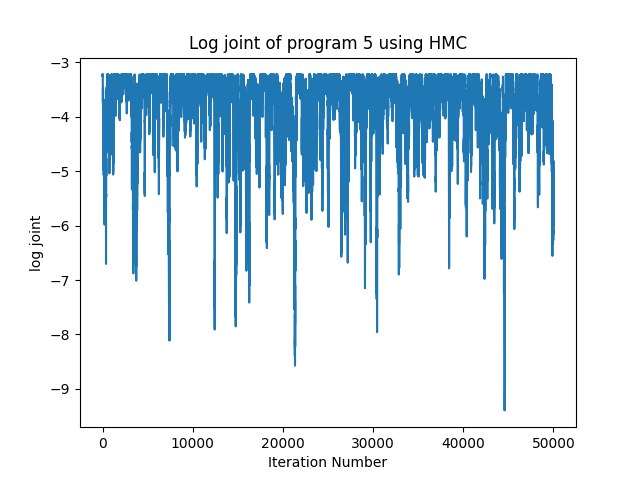
\includegraphics[width=.9\linewidth]{/home/jsefas/probprog/cpsc532w-hw2/joint-density-5-HMC.png}
\end{center}
\begin{center}
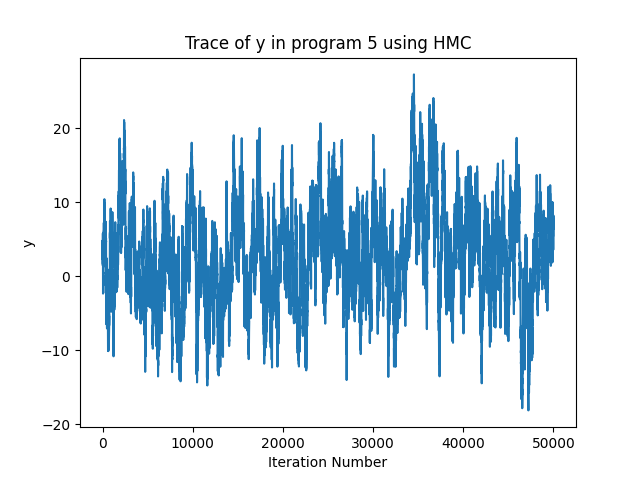
\includegraphics[width=.9\linewidth]{/home/jsefas/probprog/cpsc532w-hw2/trace-y-5-HMC.png}
\end{center}
\begin{center}
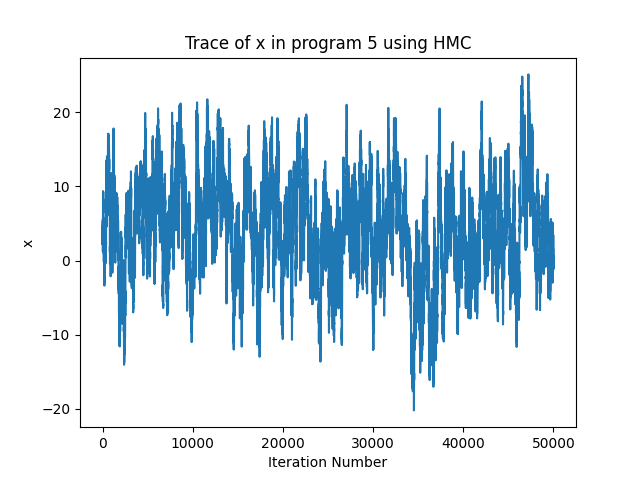
\includegraphics[width=.9\linewidth]{/home/jsefas/probprog/cpsc532w-hw2/trace-x-5-HMC.png}
\end{center}

\subsection*{Gibbs}
\label{sec:org9a7b8d4}
\begin{center}
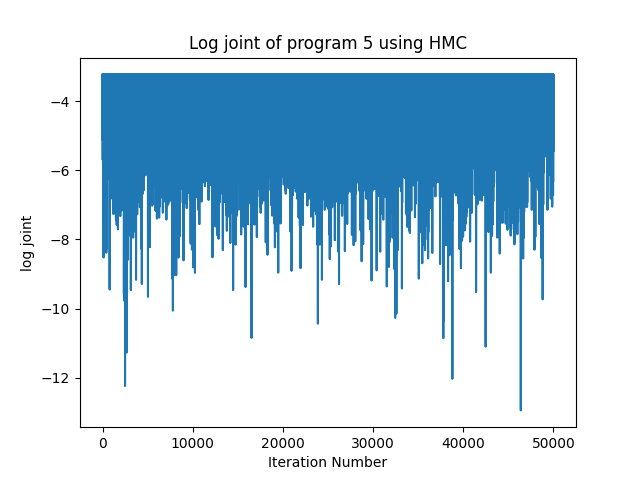
\includegraphics[width=.9\linewidth]{/home/jsefas/probprog/cpsc532w-hw2/joint-density-5-Gibbs.png}
\end{center}
\begin{center}
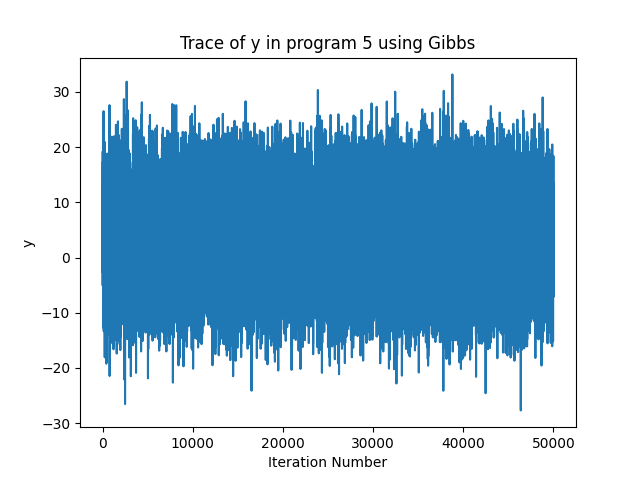
\includegraphics[width=.9\linewidth]{/home/jsefas/probprog/cpsc532w-hw2/trace-y-5-Gibbs.png}
\end{center}
\begin{center}
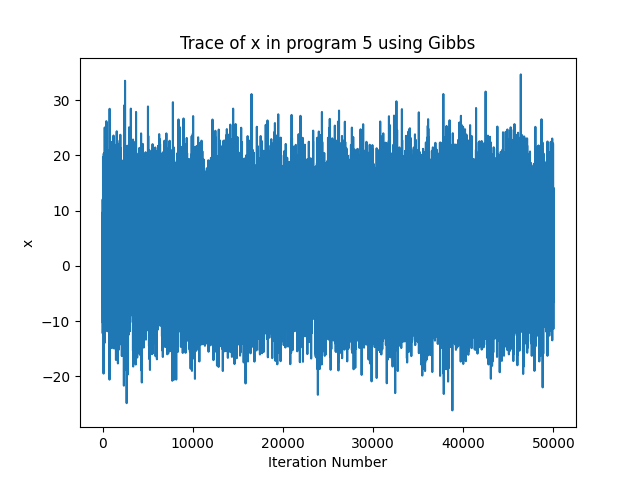
\includegraphics[width=.9\linewidth]{/home/jsefas/probprog/cpsc532w-hw2/trace-x-5-Gibbs.png}
\end{center}


\section*{Program 5}
\label{sec:orgd0702fa}
/home/jsefas/probprog/cpsc532w-hw2/trace-x-5-Importance.png      n order to solve this problem exactly, we recognize that we must sample from the line \(y=7-x\). Because \(X\) and \(Y\) are independent, their joint distribution is a spherical bivariate normal centered at the origin with diagonal variance and no covariance. Therefore any slice of this distribution is also \(\operatorname{Normal}(0,10)\), so we can simply sample from this distribution. Once we have sample \(z\sim \operatorname{N}(0,10)\), we view it as a sample from a vertical slice \(P(Y=z|X=c)\) distance \(c\) to the right of the y-axis where \(c\) is the length from the origin to the point \((3.5, 3.5)\) on \(y=7-x\). The sample we get from \(z\) defines a point in the line \(x=c\) at \([c\; z]\). We then rotate this vector \(\pi/4\) back onto the line \(y=7-x\) in order to recover our samples for \(x\) and \(y\). In particular, our equations are \(x = \dfrac{7}{2} - \dfrac{\sqrt{2}{z}{2}\) and \(y = \dfrac{7}{2} + \dfrac{\sqrt{2}{z}{2}\).

\section*{Code}
\label{sec:orgc7ca9c6}
\subsection*{Evaluation Based Importance Sampling}
\label{sec:org6797f68}
\begin{minted}[]{python}
# observe expression
if isinstance(ast, list) and 'observe' in ast:
    if 'observe' == ast[0]:
        d, sigma = eval(ast[1], sigma, local_v)
        c, sigma = eval(ast[2], sigma, local_v)
        sigma['logW'] += d.log_prob(c)
        return c, sigma
\end{minted}

\subsection*{Graph Based Gibbs Sampling and HMC}
\label{sec:orgfea62e2}
\begin{minted}[]{python}
def sample_initial(graph):
    samples, local_v = sample_from_joint(graph)
    return local_v

def computeU_old(X: torch.tensor, var_names: List[str], Y: dict, P: dict, sigma: dict):
    U = torch.tensor([0.0])
    local_map = {**{k:v for k,v in zip(var_names, X)}, **Y}
    for name, value in {k:v for k,v in zip(var_names, X)}.items():
        U -= eval(P[name][1], sigma, local_map)[0].log_prob(value)
    for name, value in Y.items():
        U -= eval(P[name][1], sigma, local_map)[0].log_prob(value)
    return U

def diffU_old(X: torch.tensor, var_names: List[str], Y: dict, P: dict, sigma: dict):
    U = computeU_old(X, var_names, Y, P, sigma)
    U.backward()

def updateR(R, eps, Xt):
    diffU(X, Y, P, sigma)
    for key in R.keys():
        R[key] = R[key] - (1/2)*eps*Xt[key].grad
        Xt[key].grad.data.zero_()
    return R

def leapfrog_old(X: torch.tensor, var_names: List[str], Y: dict, P: dict, R: torch.tensor, sigma: dict, T: int, eps: float):
    Xt = X

    diffU_old(Xt, var_names, Y, P, sigma)
    R_half = R - (1/2)*eps*Xt.grad
    Xt.grad.data.zero_()

    for t in range(1, T):
        Xt.data = Xt.data + eps*R_half

        diffU_old(Xt, var_names, Y, P, sigma)
        R_half -= eps*Xt.grad
        Xt.grad.data.zero_()

    Xt.data = Xt.data + eps*R_half

    diffU_old(Xt, var_names, Y, P, sigma)
    Rt = R_half - (1/2)*eps*Xt.grad
    Xt.grad.data.zero_()

    return Xt, Rt

def H(X, R, M, var_names, Y, P, sigma):
    return computeU_old(X, var_names, Y, P, sigma) + (1/(2*M))*torch.square(R).sum()

def hmc_sample(graph, S):
    "This function does HMC sampling"
    G = graph[1]
    P = G['P']
    Y = G['Y']
    A = G['A']
    V = G['V']
    sigma = {'logW': 0}

    local_v = sample_initial(graph)

    observeds = Y.keys()
    var_names = [v for v in V if v not in observeds]

    Y = {key: torch.tensor([value], requires_grad=False) for key, value in Y.items()}
    X = torch.tensor([value for key, value in local_v.items() if key in var_names], requires_grad=True)

    return hmc(X, var_names, Y, P, sigma = {'logW':0}, S=S)

def hmc(X: torch.tensor, var_names: List, Y: dict, P: dict, sigma: dict,
        T: int = 10, eps: float = 0.1, M: float = 1.0, S: int=10000):
    local_vars = []
    Xs = X
    for s in range(S):
        Rs = dist.MultivariateNormal(torch.zeros(len(Xs)), M*torch.eye(len(Xs))).sample([1]).reshape(-1)
        Xprime, Rprime = leapfrog_old(Xs, var_names, Y, P, Rs, sigma, T, eps)
        if torch.rand(1) < torch.exp(-H(Xprime, Rprime, M, var_names, Y, P, sigma) + H(Xs, Rs, M, var_names, Y, P, sigma)):
            Xs = Xprime
        local_vars.append({var_name: value for var_name, value in zip(var_names, X)})
    return local_vars

def accept(x: str, new_map: dict, old_map: dict, P: dict, A: dict, sigma: dict):
    """ Computes acceptance probability for MH
    arg x: name of newly proposed variable
    arg new_map: map from variable names to sample values with the new proposal value for x
    arg old_map: map from variable names to sample values with the old proposal value for x
    return: MH acceptance probability
    """
    # prior distribution
    d, sigma = eval(P[x][1], sigma, old_map)
    # prior distribution (I don't see how this can be different from d)
    d_prime, sigma = eval(P[x][1], sigma, new_map)

    # compute proposal ratio
    # (1) *given* the *new* value of x (from d_prime) calculate the probability of the *old value* (from old_map[x])
    # (2) *given* the *old* value of x (from d) calculate the probability of the *new value* (from new_map[x])
    # loga = (1) - (2)
    loga = d_prime.log_prob(old_map[x]) - d.log_prob(new_map[x])

    # get nodes where x is a parent
    vx = A[x] + [x]

    # compute posterior probability
    for v in vx:
        d1, sigma = eval(P[v][1], sigma, new_map)
        log_update_pos = d1.log_prob(new_map[v])

        d2, _ = eval(P[v][1], sigma, old_map)
        log_update_neg = d2.log_prob(old_map[v])

        loga = loga + log_update_pos - log_update_neg
    return np.exp(loga)


def gibbs_step(old_map: dict, unobserveds: List[str], P: dict, A: dict, sigma: dict):
    for x in unobserveds:
        d, sigma = eval(P[x][1], sigma, old_map)
        new_map = old_map.copy()
        new_map[x] = d.sample()
        alpha = accept(x, new_map, old_map, P, A, sigma)
        if torch.rand(1) < alpha:
            old_map = new_map.copy()
    return old_map


def gibbs_sample(graph, S = 100000):
    "This function does MH for each step of Gibbs sampling."
    G = graph[1]
    P = G['P']
    Y = G['Y']
    A = G['A']
    V = G['V'].copy()
    sigma = {'logW': 0}

    local_v = sample_initial(graph)

    observeds = Y.keys()
    unobserveds = [v for v in V if v not in observeds]

    samples: List[dict] = [local_v]
    for s in range(S):
        local_v = gibbs_step(local_v, unobserveds, P, A, sigma)
        samples.append(local_v)

    return samples
\end{minted}
\end{document}
